%=============================================================================%
% Author: 	John Joseph Valletta
% Date: 	09/04/2019
% Title: 	Fews slides on dimensionality reduction
%=============================================================================%

% Preamble
 \documentclass[pdf]{beamer}
\usepackage[export]{adjustbox}
\usepackage{framed}
\usepackage{color}
\definecolor{dkgreen}{rgb}{0,0.6,0}
\definecolor{gray}{rgb}{0.5,0.5,0.5}
\definecolor{mauve}{rgb}{0.58,0,0.82}
\definecolor{deepblue}{rgb}{0,0,0.5}
\definecolor{deepred}{rgb}{0.6,0,0}
\definecolor{deepgreen}{rgb}{0,0.5,0}
\definecolor{lightgray}{rgb}{0.92,0.92,0.92}
\definecolor{myblue}{rgb}{0.12, 0.47, 0.71} 
\definecolor{tealblue}{rgb}{0, 0.5, 0.5}
\usepackage{listings} % to insert code
\usepackage{textpos} % textblock
\usepackage{verbatim}
\usepackage{hyperref}
\hypersetup{colorlinks=true, urlcolor=blue, linkcolor=black} 

% Presentation configuration
\mode<presentation>{\usetheme{Madrid}}
\usecolortheme[named=myblue]{structure}
\useinnertheme{circles} % circles, rectanges, rounded, inmargin
\usefonttheme[onlymath]{serif} % makes math fonts like the usual LaTeX ones
\setbeamercovered{transparent=4} % transparent
\setbeamertemplate{caption}{\raggedright\insertcaption\par} % Remove the word "Figure" from caption %\setbeamertemplate{caption}[default]
\setbeamertemplate{navigation symbols}{} % don't put navigation tools at the bottom (alternatively \beamertemplatenavigationsymbolsempty)
\graphicspath{ {./img/} }

% Titlepage
\title[Dimensionality Reduction]{Dimensionality Reduction}
%\subtitle{Built-in data types}
\author{John Joseph Valletta}
\date[April 2019]{April 2019}
\institute[]{University of Exeter, Penryn Campus, UK}
\titlegraphic{
\hfill

\includegraphics[width=\textwidth, keepaspectratio]{logo.jpg}}

%=============================================================================%
%=============================================================================%
% Start of Document
%=============================================================================%
%=============================================================================%
\begin{document}

%=============================================================================%
%=============================================================================%
\begin{frame}
\titlepage
\end{frame}

%=============================================================================%
%=============================================================================%
\begin{frame}{Why reduce the dimensionality of the problem?}
\begin{itemize}\addtolength{\itemsep}{2\baselineskip}
	\item<2-> Visualise the data to uncover structure
	\item<3-> Elucidate the best predictors of the underlying process (plausible causal drivers under an experimental setup)
	\item<4-> Improve the model's predictive performance by removing uninformative features/extracting better features
	\item<5-> Decrease computational power
\end{itemize}
\end{frame}

%=============================================================================%
%=============================================================================%
\begin{frame}{Dimensionality Reduction}

\begin{block}{Rationale}
Although the data may seem high dimensional, the \textbf{structure} of the data can be represented by fewer features.
\end{block}
\vfill
\visible<2->{Dimensionality reduction can be achieved through:}
\begin{itemize}\addtolength{\itemsep}{0.5\baselineskip}
	\item<3-> \textbf{Feature extraction}: mapping the original data to a new feature set
	\item<4-> \textbf{Feature selection}: selecting a subset of attributes
\end{itemize}
\end{frame}

%=============================================================================%
%=============================================================================%
\begin{frame}{Principal Component Analysis}

\begin{itemize}\addtolength{\itemsep}{1.5\baselineskip}
	\item A \textbf{linear} dimensionality reduction method
	\item The new uncorrelated features (PCA 1, PCA 2,...) are \textbf{weighted} ($w$'s) linear combinations of the original data ($x$'s)
	\begin{align*}
	\text{PCA 1} &= w_{11}x_1 + w_{12}x_2 + \ldots + w_{1p}x_p\\
	\text{PCA 2} &= w_{21}x_1 + w_{22}x_2 + \ldots + w_{2p}x_p\\
	& \vdots\\ 
	\text{PCA p} &= w_{p1}x_1 + w_{p2}x_2 + \ldots + w_{pp}x_p
	\end{align*}
	\item Objective is to find directions, called principal components, that maximise the variance of the data
\end{itemize}
\end{frame}

%=============================================================================%
%=============================================================================%
\begin{frame}{Principal Component Analysis}
	\begin{center}
		\includegraphics<1>[width=0.7\textwidth]{03-pca00.png}
		\includegraphics<2>[width=0.7\textwidth]{03-pca01.png}
		\includegraphics<3>[width=0.7\textwidth]{03-pca02.png}
	\end{center}
\end{frame}

%=============================================================================%
%=============================================================================%
\begin{frame}{t-Distributed Stochastic Neighbor Embedding (t-SNE) }
\begin{itemize}\addtolength{\itemsep}{2\baselineskip}
	\item A \textbf{non-linear} dimensionality reduction method
	\item Projects data into a lower-dimensional space/embedding such that the original high-dimensional clustering is preserved 
\end{itemize}

\end{frame}

%=============================================================================%
%=============================================================================%
\begin{frame}{t-SNE on handwritten digits}
\centering
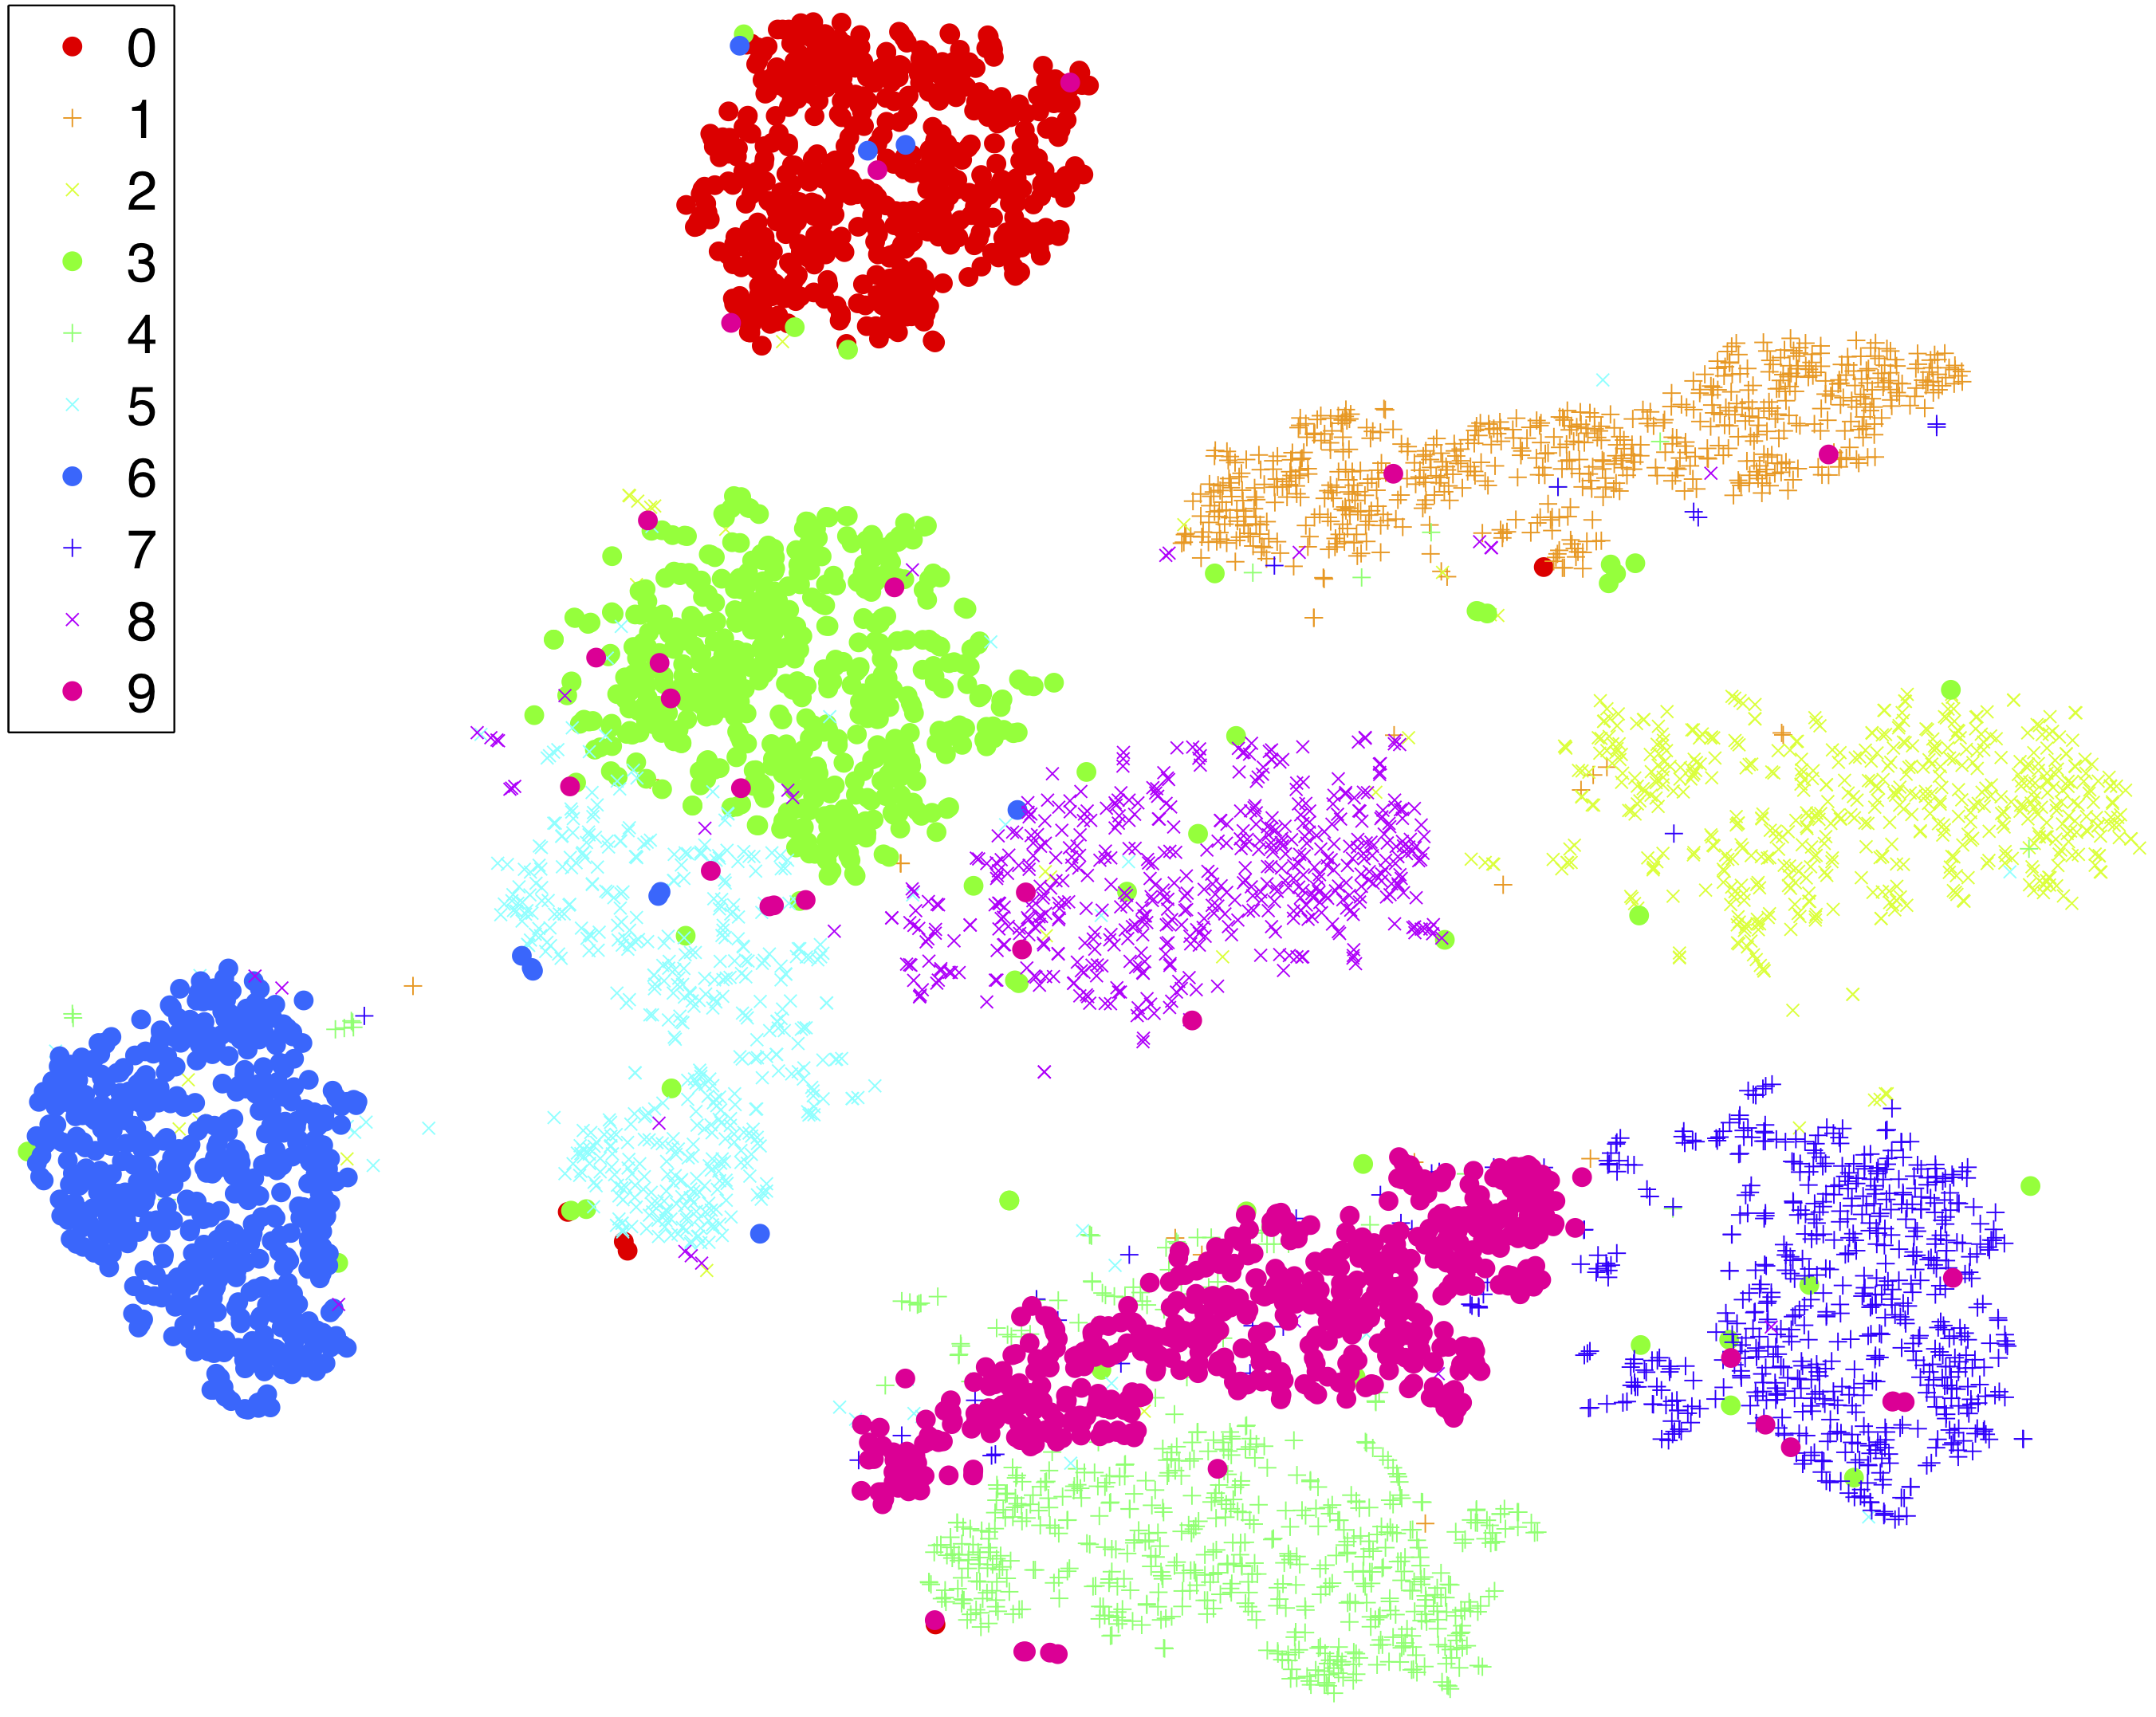
\includegraphics[width=0.7\textwidth]{03-mnist.png}
\vfill
{\tiny L. Van der Maaten and G. Hinton. (2008) \textit{Journal of Machine Learning Research}}
\end{frame}

%=============================================================================%
%=============================================================================%
\begin{frame}{t-SNE on flow cytometry data}
\centering
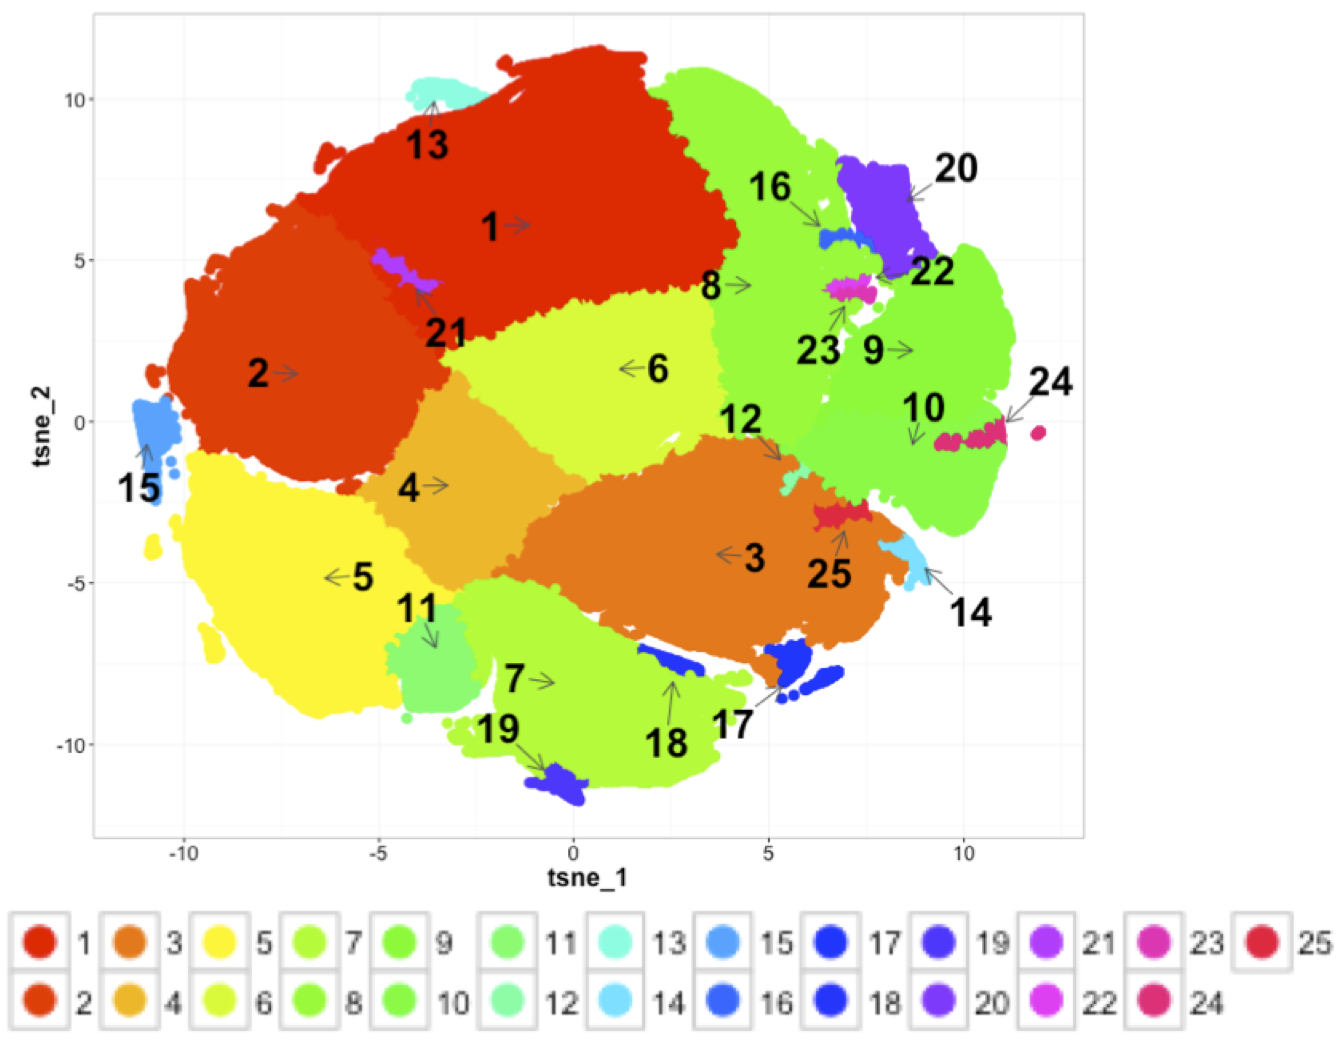
\includegraphics[width=0.7\textwidth]{03-flow.png}
\vfill
{\tiny Y. Bediako, R. Adams, A. Reid, J.J. Valletta, F. Ndungu \textit{et al}. (2019) \textit{BMC Medicine}}
\end{frame}

%=============================================================================%
%=============================================================================%
\begin{frame}{Comparison of methods}
\centering
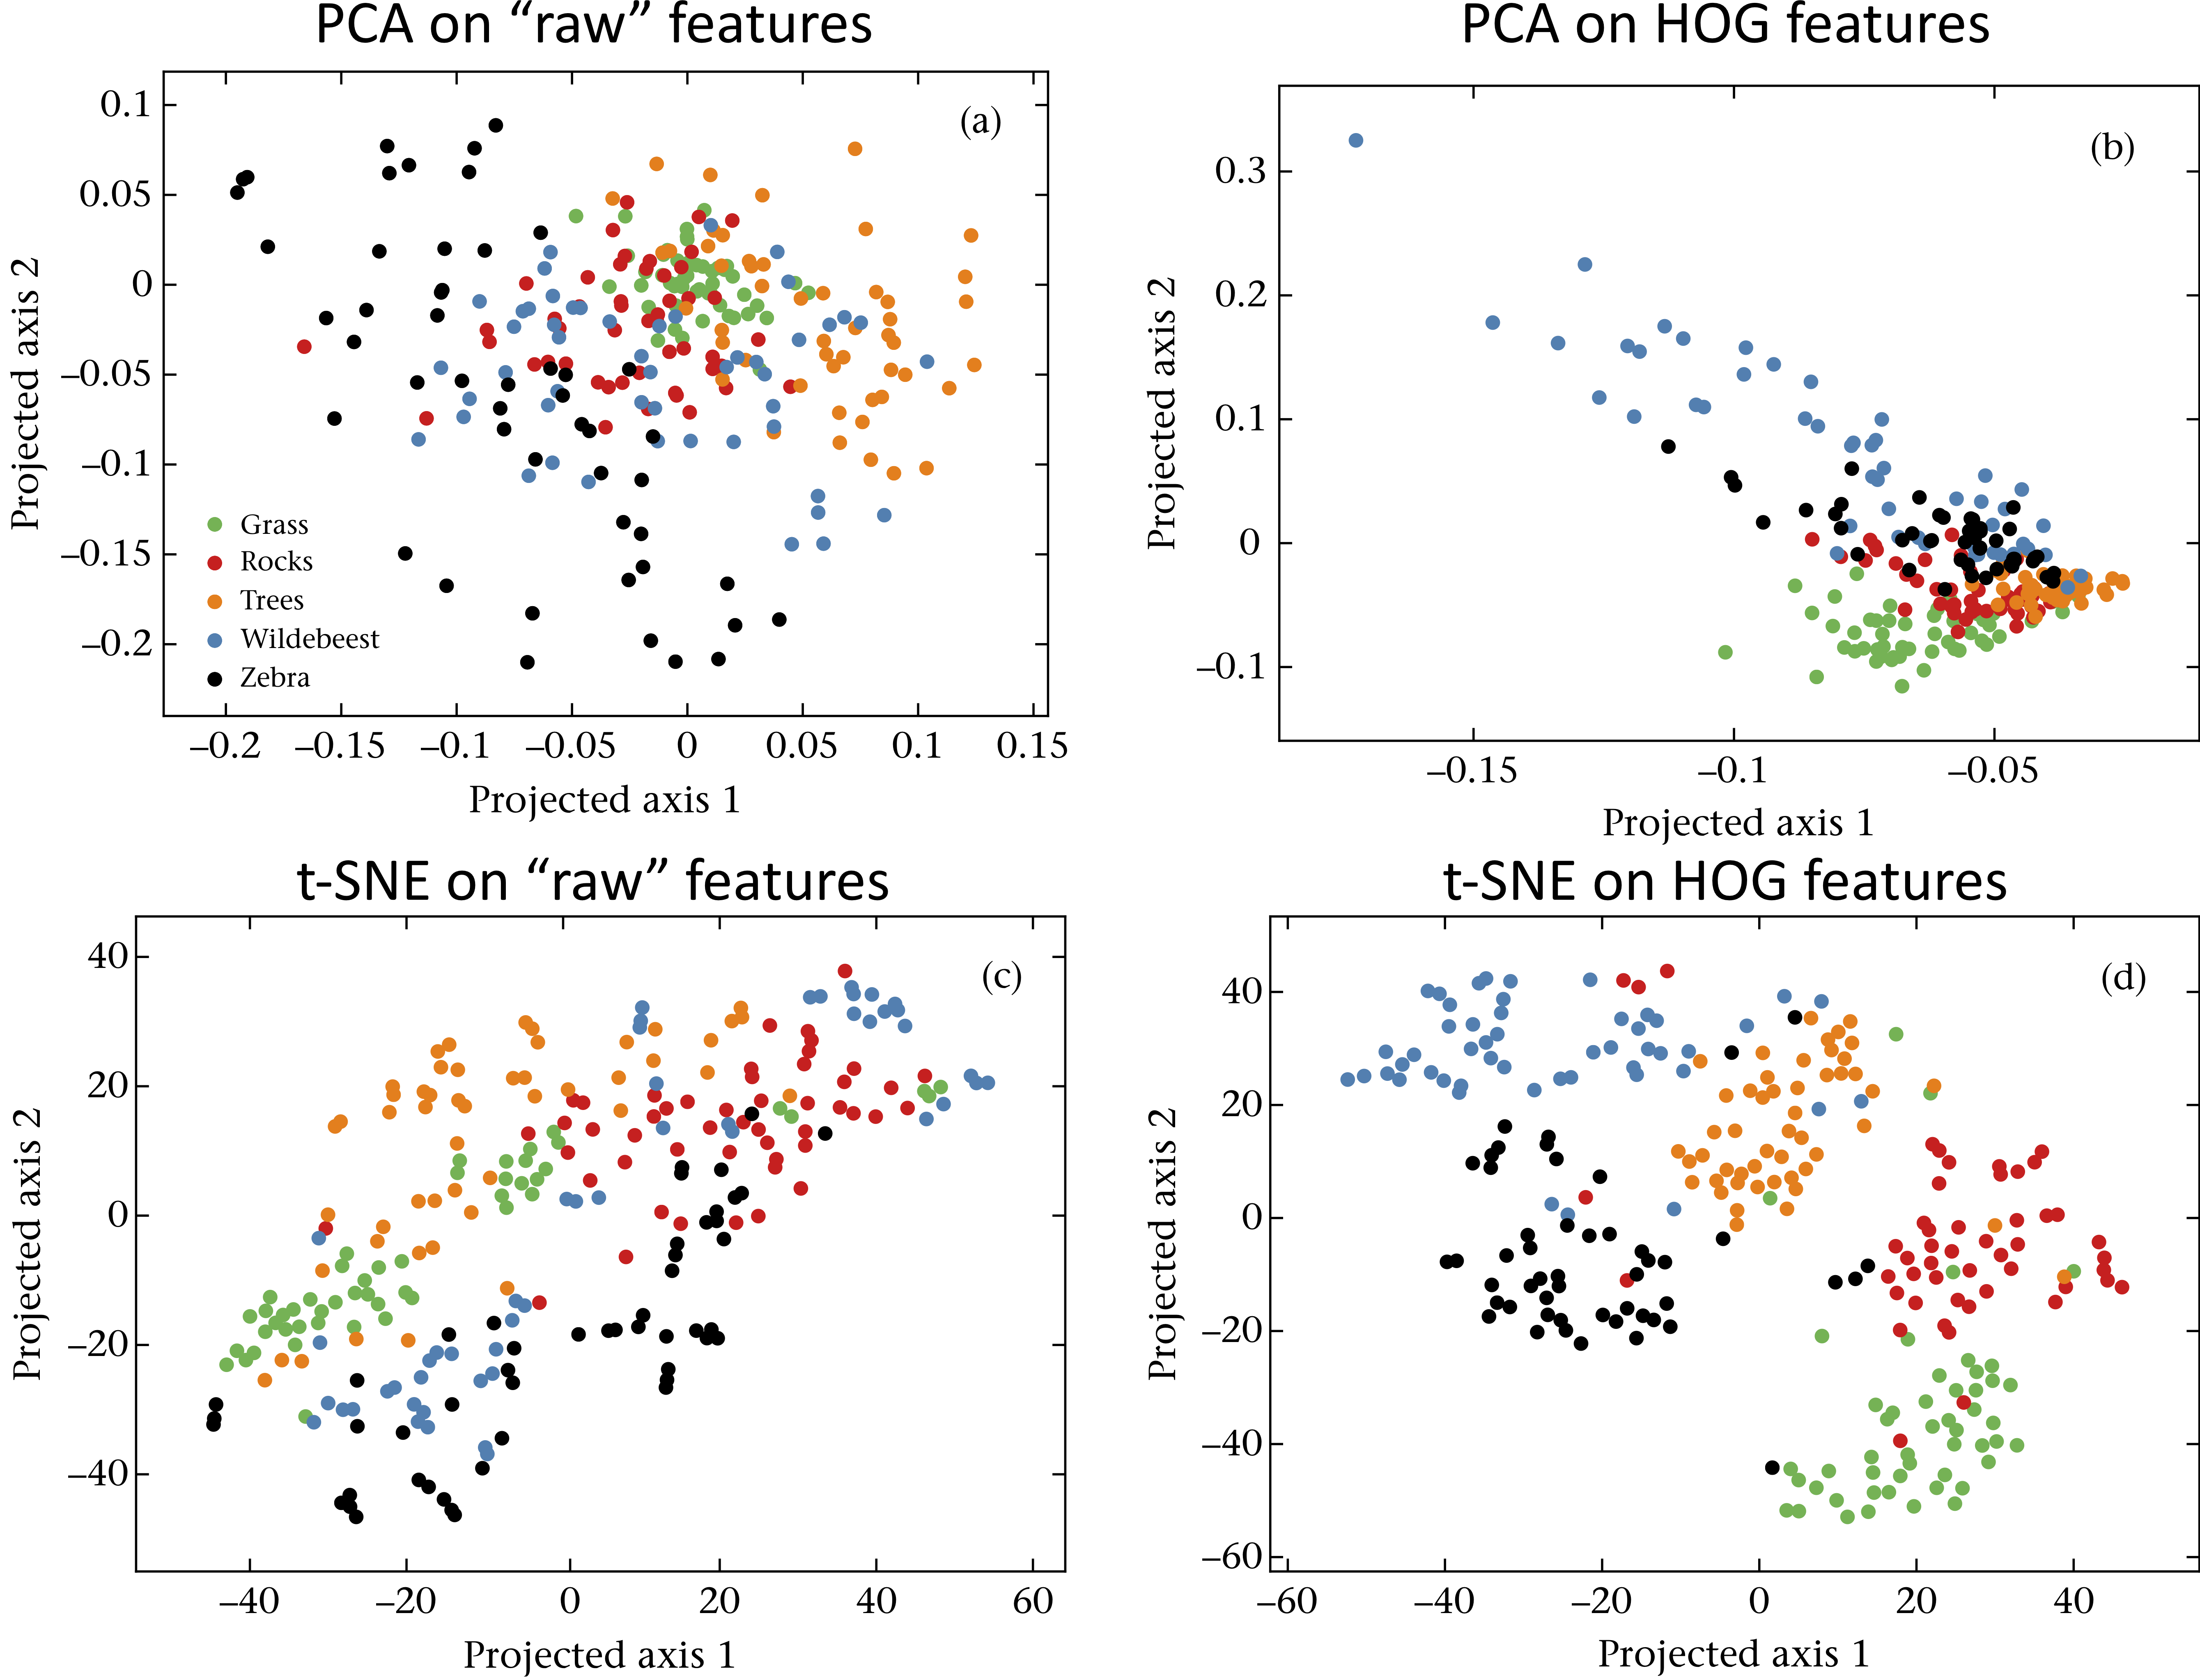
\includegraphics[width=.75\textwidth]{03-comparison.png}
\vfill
{\tiny J.J. Valletta \textit{et al}. (2017) \textit{Animal Behaviour}}
\end{frame}


%=============================================================================%
%=============================================================================%
\end{document}
%=============================================================================%
%=============================================================================%
% End of Document
%=============================================================================%
%=============================================================================%